\section{FlashAttention 4 and asymmetric hardware scaling}
\label{sec:C04:frontier}
FlashAttention-4 addresses Blackwell through a redesigned asynchronous pipeline, tensor-memory use, software-assisted exponentials, and a two-CTA backward strategy. Its Section 5 reports B200 BF16 results up to 1613 TFLOPs/s, with maxima of $1.3\times$ against cuDNN 9.13 and $2.7\times$ against its Triton comparator. The paper's Figure 4 also states that newer cuDNN versions incorporated related techniques and reached similar performance~\cite{rewrite_fa4}. Those version-qualified observations rule out using the original maximum as a timeless vendor-library ranking.

The pinned forward class is \texttt{FlashAttention\allowbreak ForwardSm100} in \path{flash_attn/cute/flash_fwd_sm100.py}, with \path{mma_ping_pong_qk}, \path{softmax_loop}, and \path{correction_loop}; \texttt{FlashAttention\allowbreak BackwardSm100} is in the corresponding backward module~\cite{repo_flashattention}. The important comparison with FA3 is the placement and overlap of work on hardware resources, not a different semantic attention objective. A faster matrix engine can leave exponentials or shared-memory traffic dominant. A correction stage removed from a critical path can help even when total arithmetic remains similar. This is why counting FLOPs alone can miss the mechanism of a kernel improvement.

An independent resource model makes the implication explicit. Let a tile require matrix time $t_m$, nonlinear time $t_s$, and movement time $t_b$ on separately overlappable resources. An ideal pipeline cannot complete faster than $\max(t_m,t_s,t_b)$ per steady-state tile. Doubling only matrix throughput replaces $t_m$ by $t_m/2$; when $t_s$ already exceeds $t_m/2$, the full twofold gain is impossible without changing nonlinear work or overlap. This deduction does not require assigning an invented bandwidth to B200. It explains which measured counters could falsify a proposed bottleneck account.

Software approximations of elementary functions additionally need numerical auditing. The relevant comparison includes error before and after conversion to the attention input precision, extremes of the logit distribution, and repeated long-sequence reductions. Approximation of an exponential within an implementation is different from removing attention positions. Both can alter output, but their error models differ. A code review should trace the selected architecture, dtype, head dimensions, and compile-time options to the actual path rather than assuming that installation of a library guarantees a particular kernel executes.

For agent serving, benchmark the selected FA4 path under both large prefills and the service's actual decode shapes, then inspect end-to-end task latency. Preserve a versioned cuDNN or alternative comparator, because a later library update can absorb the same optimization. Separate compilation time from execution time when evaluating a DSL-based implementation: faster iteration can be valuable even when steady-state kernel throughput is matched. None of these measurements establish better long-context reasoning without a quality test. The kernel contribution is reduced cost of a specified computation; the agent contribution is what useful decisions that computation enables under the released resource budget.



% SCIENTIFIC_FIGURE_C04
Figure~\ref{fig:C04:overview} distinguishes evaluation of the same target attention operator from logical-to-physical cache allocation.
\begin{figure}[!htbp]
\centering
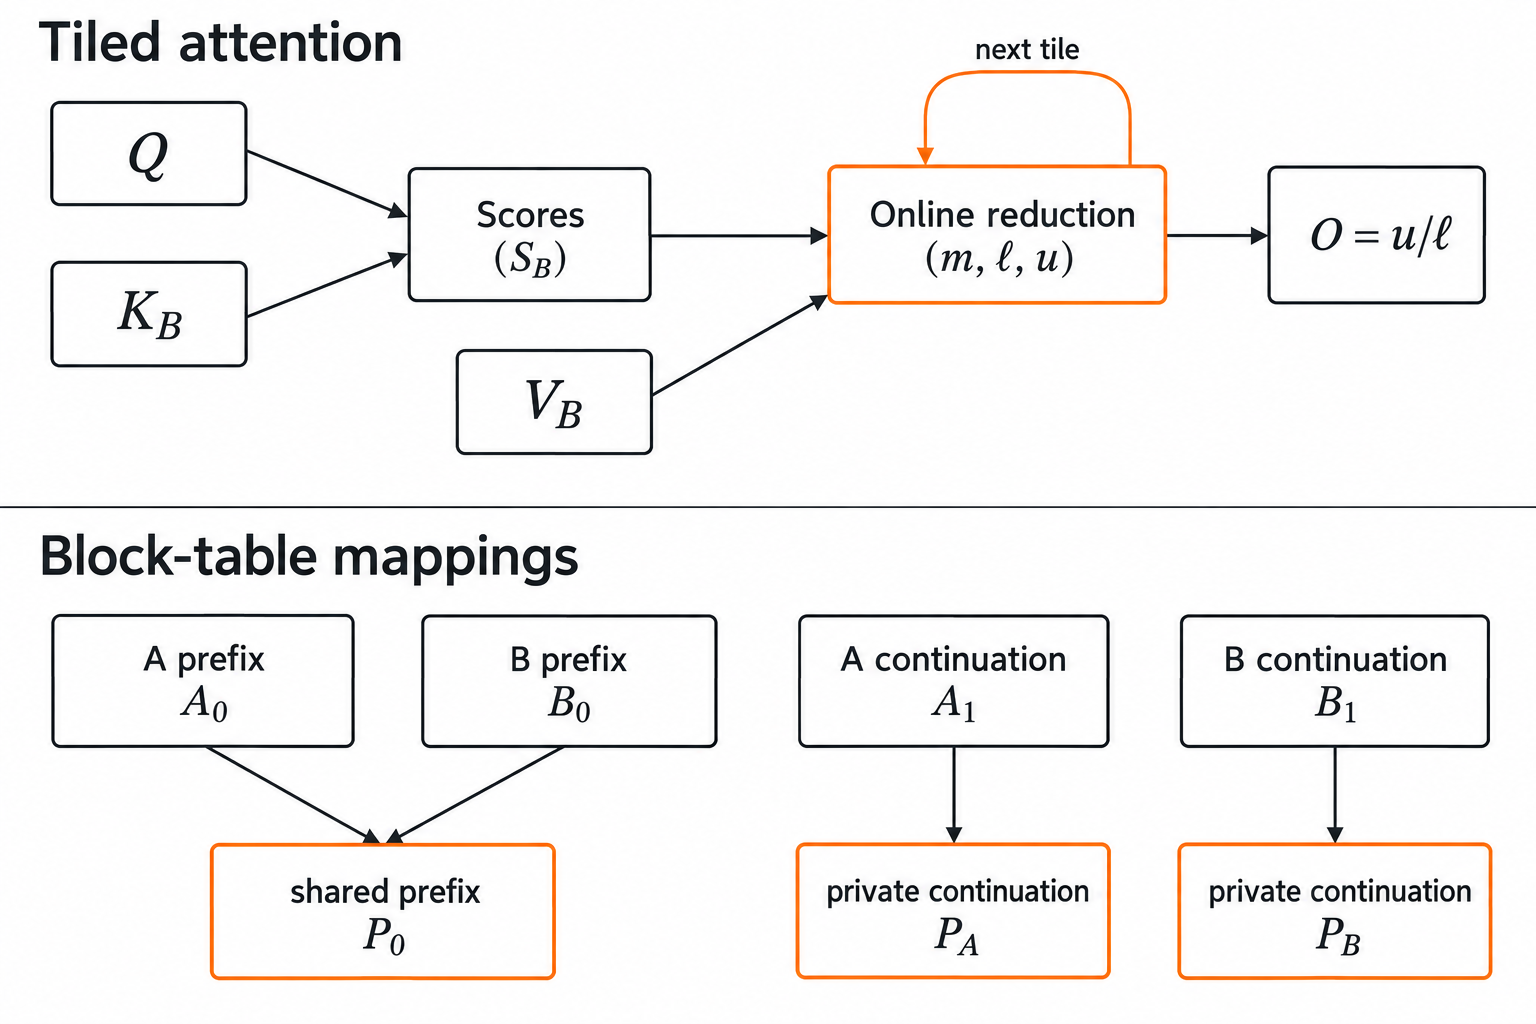
\includegraphics[width=\linewidth]{book/figures/assets/F04review.png}
\caption{Tiled reduction and paged allocation preserve different objects. Top: query, key and value tiles update the running maximum $m$, normalizer $\ell$ and weighted-value sum $u$; normalization forms $O=u/\ell$ for a nonempty visible row. Bottom: block tables can share a complete eligible prefix while mapping divergent continuations to different physical storage. The lower arrows are allocation mappings, not attention edges. No performance measurements are depicted.}
\label{fig:C04:overview}
\end{figure}
